\titleformat{\chapter}[display]
{\normalfont\huge\bfseries}{Capítulo \thechapter}{0.5em}{\huge}
\titlespacing*{\chapter}{0pt}{-1.25cm}{25pt}
\chapter{Propuesta de la Idea}

\section{Requisitos}

La solución propuesta debe cumplir con una serie de requisitos imprescindibles para asegurar su utilidad y accesibilidad:

\begin{itemize}
    \item \textbf{Bajo Costo:} La solución debe ser económica para garantizar su accesibilidad a una amplia gama de usuarios, incluidos aquellos con presupuestos limitados.
    
    \item \textbf{Flexibilidad de Alojamiento:} La solución debe ofrecer la capacidad de auto-alojamiento, los usuarios deben poder optar por alojarla en sus propios servidores o usar la solución en la nube según sus preferencias y requisitos específicos.
    
    \item \textbf{Extensible:} La solución debe ser extensible, lo que significa que debe permitir la integración de nuevas funcionalidades y la expansión de su capacidad según las necesidades cambiantes de los usuarios.
    
    \item \textbf{Mejor Filtrado:} Se debe ofrecer un filtrado más preciso y flexible en comparación con las plataformas existentes, lo que permitirá a los usuarios obtener información relevante y útil de los datos APRS para complementar la ya provista por las alternativas.
    
	\item \textbf{Análisis de Datos Integrado:} La solución debe incluir un análisis de datos integrado para ayudar a los usuarios a comprender mejor la información recibida a través del APRS y obtener perspectivas y conclusiones valiosas a partir de los mensajes transmitidos.
	
\end{itemize}

\section{La Idea}
Se propone una solución completa que incluya la adquisición, procesamiento, visualización y análisis de datos APRS. La solución se centrará en mejorar la experiencia del usuario y enriquecer la información disponible a través de la integración de datos de diversas fuentes abiertas y disponibles.

\subsection{Enfoque}

\begin{itemize}
    \item \textbf{Experiencia de Usuario Mejorada:} La solución tendrá una interfaz intuitiva, rápida y útil que facilite la navegación y la interacción con los datos.
    
    \item \textbf{Análisis avanzado:} La solución contará con herramientas avanzadas para la visualización detallada del tráfico APRS, filtrado preciso y análisis de datos, con el objetivo de extraer inteligencia de los mensajes recibidos.
    
    \item \textbf{Complementación:} La solución no tiene como objetivo sustituir a aprs.fi, aprs.to u otras plataformas similares, sino ofrecer una alternativa con funcionalidades complementarias que enriquezcan la experiencia del usuario.
    
    \item \textbf{Enriquecimiento de Información:} Se recopilarán datos provenientes de diversas fuentes abiertas y disponibles para ofrecer una visión más completa del tráfico APRS y sus usuarios, mejorando así la calidad de la información disponible para los usuarios.
\end{itemize}

\subsection{Beneficios}

\begin{itemize}
    \item \textbf{Mayor Comprensión del Tráfico APRS:} Los usuarios podrán obtener información más detallada y procesable a partir de los mensajes transmitidos, lo que les permitirá una mayor comprensión del tráfico APRS.
    
	\item \textbf{Toma de Decisiones más Efectiva:} El análisis de datos integrado ayudará a los usuarios a tomar decisiones más informadas en base a la información recibida, mejorando así la eficacia de sus acciones.
    
    \item \textbf{Flexibilidad:} La opción de autoalojamiento permitirá a los usuarios tener un mayor control sobre sus datos y privacidad, proporcionando así una mayor flexibilidad en cuanto a su gestión.
\end{itemize}

\section{APRSINT}
La solución propuesta se ha llamado \textbf{APRSINT}, que es una combinación de APRS y OSINT. APRSINT está dividida en tres módulos principales:
\begin{itemize}
	\item \textbf{Adquisición de Datos:} Este módulo se encargará de recopilar y almacenar los mensajes APRS de diversas fuentes, así como de integrar datos de otras fuentes abiertas y disponibles.
	\item \textbf{Procesamiento y Análisis:} Este módulo se encargará de procesar y analizar los datos recopilados, ofreciendo herramientas avanzadas de visualización, filtrado y análisis de datos.
	\item \textbf{Visualización y Presentación:} Este módulo se encargará de presentar los datos procesados y analizados de forma clara y comprensible, facilitando la interpretación y la toma de decisiones.
\end{itemize}




\begin{figure}[h]
    \centering
    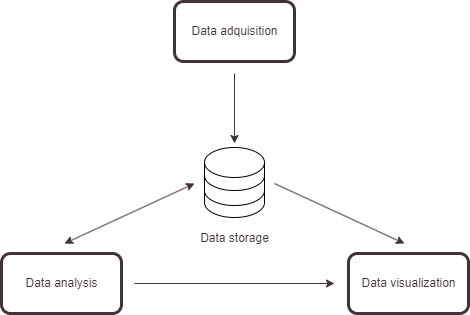
\includegraphics[width=0.85\textwidth]{./Chapter_3/structure.png}
    \caption{Estructura base de la aplicación.}
    \label{fig:aprsint-logo}
\end{figure}

Cada uno de estos módulos será explicado en detalle en el capítulo siguiente.
